% =============================================================================
% method.tex  --  drop-in replacement for \section{Method}
%
% FIGURE: figures/method.pdf  (rendered by figures/render_method.py with
%   matplotlib; a vector TikZ source for camera-ready is figures/method_fig.tex).
%   To regenerate:  python figures/render_method.py   (uses the `starVLA' env).
%   Needs only \usepackage{graphicx} (already in the main preamble).
%
% Method name: SPT = "Self-Labeled Preference Transfer". To rename globally,
%   find/replace "SPT" and the long form in the title/abstract/intro.
% =============================================================================

\section{Method}
\label{sec:method}

\begin{figure}[t]
  \centering
  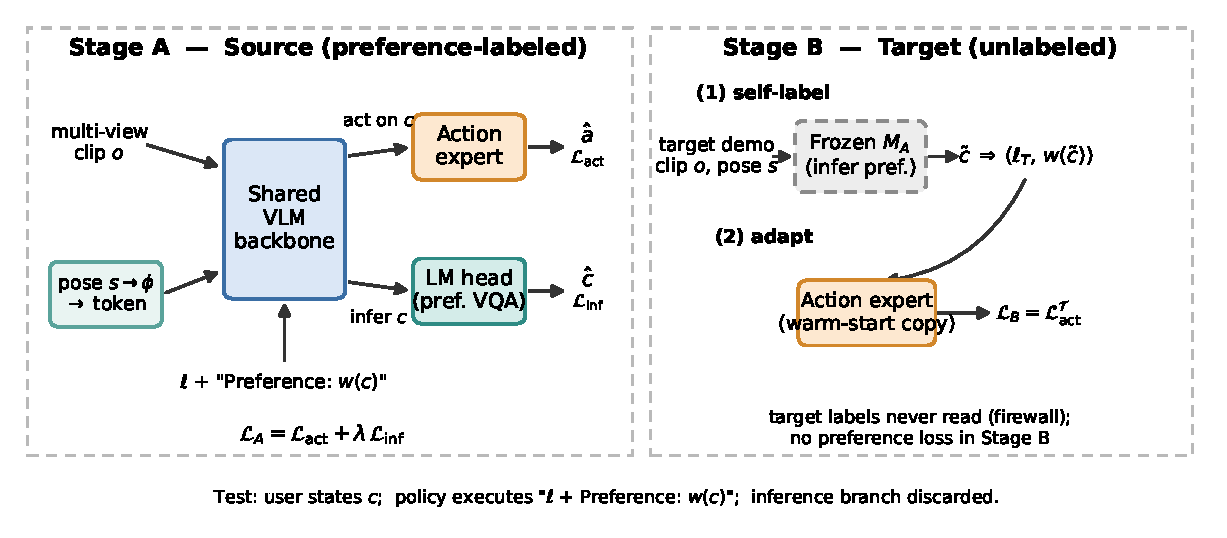
\includegraphics[width=\linewidth]{figures/method.pdf}
  \caption{\textbf{Self-Labeled Preference Transfer (SPT).} One shared VLM
  backbone serves as a policy that acts on a stated preference (\emph{act on
  $c$}) and as a head that predicts the preference of a demonstration
  (\emph{infer $c$}). The prediction head reads the VLM's language output, and
  takes the proprioceptive state as a learned token $\phi(s)$. Stage~A trains
  both on the labeled source. Stage~B freezes this model, labels each unlabeled
  target demonstration with the prediction head, and continues training the
  action expert on the labeled prompts. At test time the user sets $c$ and only
  the policy is used.}
  \label{fig:method}
\end{figure}

We build a single vision--language--action model in which one shared backbone
plays two roles. As a policy it maps an instruction and a stated preference to
an action chunk, $\pi_\theta(a\mid o,s,\ell,c)$. As a preference predictor it
maps a demonstration to the preference it exhibits,
$g_\theta(c\mid o,s)$. We train both on the labeled source. To adapt to a target
task that has demonstrations but no preference labels, we run the predictor over
the target demonstrations to recover their preferences, and then continue
training the policy on the resulting labeled prompts (Fig.~\ref{fig:method}).

\textbf{Architecture.}
The backbone is a pretrained vision--language model (VLM) that encodes the
multi-view observation, the proprioceptive state, and the text prompt. An
\emph{action expert} decodes the backbone features into a chunk of end-effector
actions. We condition it on the preference through language, appending
``Preference:~$w(c)$'' to the instruction $\ell$, where $w(c)$ is a fixed short
phrase for each preference value (e.g., ``grasp low''). For preference
prediction we add no new module: we pose a binary question about the preference
and read the answer off the VLM's language head as a single token. Because both
roles read the same backbone, training the predictor also shapes the features
the policy uses.

The preference is often only weakly visible in the camera views, so we also give
the predictor the robot's proprioceptive state. A small MLP $\phi$ encodes the
active end-effector pose over the clip into one token, which we insert into the
VLM input next to the image tokens. We pass the pose as a learned token rather
than as numeric text, which the model tends to ignore. The conditioning phrase
$w(c)$ and the answer token may differ in surface form (e.g., \emph{near}/%
\emph{far} for the question, \emph{narrow}/\emph{wide} for the prompt), as long
as both are fixed.

\textbf{Stage~A: training on the labeled source.}
We train the two roles jointly. Action samples carry the preference-conditioned
prompt $(\ell,w(c))$ and an action-regression loss
$\mathcal{L}_{\mathrm{act}}$; prediction samples carry the binary question and a
single-token cross-entropy loss $\mathcal{L}_{\mathrm{inf}}$. We optimize
\begin{equation}
  \mathcal{L}_{A} \;=\; \mathcal{L}_{\mathrm{act}} \;+\; \lambda\,\mathcal{L}_{\mathrm{inf}},
  \label{eq:stageA}
\end{equation}
which yields a source model $M_A=(\pi_{\theta_A},\,g_{\theta_A})$.

\textbf{Stage~B: adapting to the unlabeled target.}
We start from $M_A$ and use only the unlabeled target demonstrations
$\mathcal{D}_{\mathcal{T}}$. First, we label each target episode with the frozen
source predictor,
\begin{equation}
  \tilde{c}^{(j)} \;=\; \arg\max_{c\in\mathcal{C}}\; g_{\theta_A}\!\big(c \mid o^{(j)},s^{(j)}\big).
  \label{eq:pseudolabel}
\end{equation}
We never read the target's ground-truth preference; it is recovered from the
model alone. Second, we continue training the action expert on the relabeled
prompts $(\ell_T,w(\tilde{c}))$ with the action loss,
\begin{equation}
  \mathcal{L}_{B} \;=\; \mathcal{L}^{\mathcal{T}}_{\mathrm{act}}\!\big(w(\tilde{c})\big).
  \label{eq:stageB}
\end{equation}
We do not update the predictor in this stage.

\textbf{Deployment.}
On a target task the user gives a preference $c\in\mathcal{C}$ from the source
set, and the policy acts on ``$\ell$.~Preference:~$w(c)$''. The prediction head
is used only for labeling and is dropped at test time.
